\usetikzlibrary{calc}
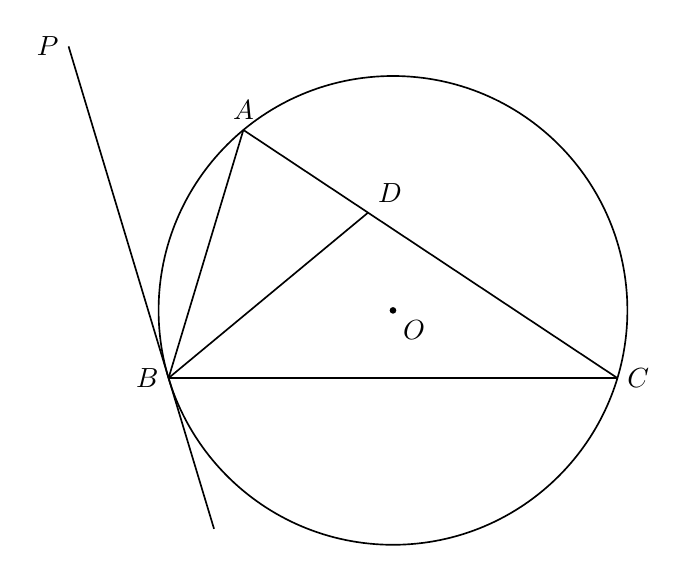
\begin{tikzpicture}[x=1cm,y=1cm,line width=.6pt,font=\normalsize]
\coordinate (B) at (0.0,0.0);
\coordinate (C) at (5.7,0.0);
\coordinate (A) at (0.95,3.15079);
\coordinate (D) at (2.53333,2.10053);
\coordinate (O) at (2.85,0.85931);
\coordinate (P) at (-1.27017,4.21268);
\coordinate (Q) at (0.57735,-1.91485);
\draw (O) circle[radius=2.97673cm];
\draw (P)--(Q);
\draw (A)--(B);
\draw (B)--(C);
\draw (A)--(C);
\draw (B)--(D);
\fill (O) circle[radius=1.2pt];
\node[left] at (P) {$P$};
\node[above] at (A) {$A$};
\node[left] at (B) {$B$};
\node[right] at (C) {$C$};
\node[above right] at (D) {$D$};
\node[below right] at (O) {$O$};
\end{tikzpicture}
